\documentclass[12pt,a4paper,fleqn]{article}
\usepackage[utf8]{inputenc}
\usepackage[russian]{babel}
\usepackage{amssymb, amsmath, multicol}
\usepackage{enumitem}
\usepackage{lipsum}
\usepackage{euler}
\oddsidemargin=-15.4mm
\textwidth=190mm
\headheight=-32.4mm
\textheight=277mm
\parindent=0pt
\parskip=8pt
\pagestyle{empty}
\usepackage{graphicx}
\title{\textbf{\LARGE{Исследовательская работа по теме:\\Исследование функции дифференциальными методами}}}
\author{Известный гражданин}
\date{November 2022}
\addt\captionsrussian{\def\refname{Список литературы}}\begin{document}
\maketitle
\newpage\newpage \textbf{\LARGE{Глава I. Функция}}

\begin{center}
$y = $$3 \cdot cos(x)$

\end{center}
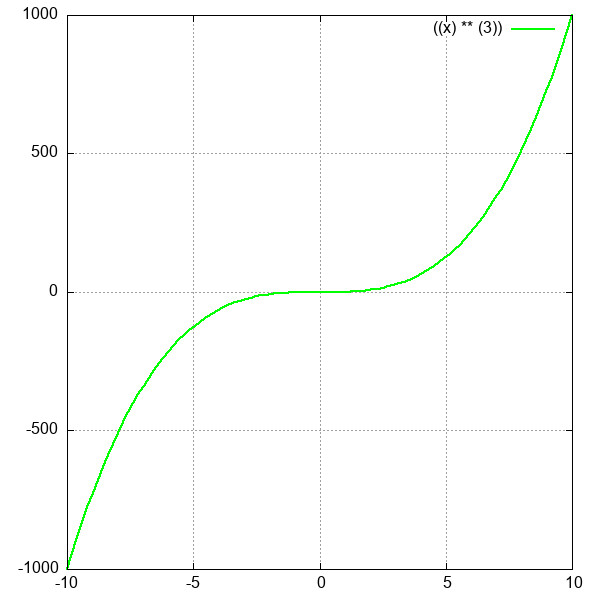
\includegraphics{GraphicDumps/plot.jpg}\newpage \textbf{\LARGE{Глава II. Визуальный анализ функции}}

Для любого эпсилон больше нулю очевидно, что

\begin{center}
$y = $$3 \cdot cos(x)$

\end{center}
\newpage \textbf{\LARGE{Глава III. Дифференцирование}}

Положим

\begin{center}
 ($3)'
  = 0$\end{center}
[Данные удалены]

\begin{center}
 ($x)'
  = 1$\end{center}
Говорят

\begin{center}
 ($cos(x))'
  = 1 \cdot (0-sin(x))$\end{center}
Господи, да для кого я вообще стараюсь

\begin{center}
 ($3 \cdot cos(x))'
  = 0 \cdot cos(x)+3 \cdot (1 \cdot (0-sin(x)))$\end{center}
DUMP

$0 \cdot cos(x)+3 \cdot (1 \cdot (0-sin(x)))$DUMP
\newpage \textbf{\LARGE{Глава IV.Упрощение выражения}}

В ближайшее время ожидаются осадки из ваших слёз от попыток понять этот переход

\begin{center}
$0 \cdot cos(x) = 0$\end{center}
Откуда

\begin{center}
$1 \cdot (0-sin(x)) = 0-sin(x)$\end{center}
По теореме Эскобара

\begin{center}
$0+3 \cdot (0-sin(x)) = 3 \cdot (0-sin(x))$\end{center}
\newpage \textbf{\LARGE{Глава V. Полученая производная}}

$y = $$3 \cdot cos(x)$

$y' = $$3 \cdot (0-sin(x))$

\includegraphics{GraphicDumps/plot_1.jpg}\newpage \textbf{\LARGE{Глава VI. Разложение функции по формуле Тейлора}}

Ты же продолжаешь читать, да?

\begin{center}$cos(0) = 1$\end{center}
Поэтому

\begin{center}$3 \cdot 1 = 3$\end{center}
Оказывается

\begin{center}
 ($3)'
  = 0$\end{center}
Я придумал поистине удивительное доказательство этого факта, но поля этой книги слишком малы\ldots

\begin{center}
 ($x)'
  = 1$\end{center}
Не трудно заметить

\begin{center}
 ($cos(x))'
  = 1 \cdot (0-sin(x))$\end{center}
Вычислительные ошибки уйдут, достаточно просто...

\begin{center}
 ($3 \cdot cos(x))'
  = 0 \cdot cos(x)+3 \cdot (1 \cdot (0-sin(x)))$\end{center}
Имеем

\begin{center}
$0 \cdot cos(x) = 0$\end{center}
Ну ты же всё равно не будешь это проверять

\begin{center}
$1 \cdot (0-sin(x)) = 0-sin(x)$\end{center}
В ближайшее время ожидаются осадки из ваших слёз от попыток понять этот переход

\begin{center}
$0+3 \cdot (0-sin(x)) = 3 \cdot (0-sin(x))$\end{center}
Нам не объяснили на семинаре как это делать, поэтому примем на веру

\begin{center}$sin(0) = 0$\end{center}
Не так страшна производная, как её находят\cite{link2}

\begin{center}$0-0 = 0$\end{center}
И хотя клуб любителей таких формул двумя блоками ниже, мы продолжаем

\begin{center}$3 \cdot 0 = 0$\end{center}
Так как 1=1, то\cite{link4}

\begin{center}$\frac{0}{1} = 0$\end{center}
Как было показано ранее

\begin{center}
$x-0 = x$\end{center}
Если вы понимаете данный переход, то я вам сочувствую

\begin{center}
$x^{1} = x$\end{center}
Паршивая функция всё доказательство портит\cite{link2}

\begin{center}
$0 \cdot x = 0$\end{center}
Производная дураков любит\cite{link2}

\begin{center}$3+0 = 3$\end{center}
\textbf{\LARGE{Получим разложение по формуле Тейлора:}}
\begin{center}
$y = $$3$$ + o((x - 0.000000)^{1})$
\end{center}
\newpage\begin{thebibliography}{}
\bibitem{link1}  "A Synopsis of Elementary Results in Pure and Applied Mathematics"
\bibitem{link2}  "Сборник пословиц и поговорок под редацией кафедры высшей математики"
\bibitem{link3}  "Полное собрание лучших высказываний преподавателей МФТИ"
\bibitem{link4}  "Словарь фраз, не несущих смысловой нагрузки. 17 издание"
\end{thebibliography}\end{document}